
%(BEGIN_QUESTION)
% Copyright 2011, Tony R. Kuphaldt, released under the Creative Commons Attribution License (v 1.0)
% This means you may do almost anything with this work of mine, so long as you give me proper credit

Suppose we encounter a differential pressure transmitter used to measure pressure drop across a heat exchanger.  The typical pressure on the upstream side of this heat exchanger is 850 PSI, while the typical pressure on the downstream side of this exchanger is 837 PSI.  The transmitter connects to this heat exchanger via a three-valve manifold.  A single ``bleed'' valve installed on the transmitter's low-pressure side is used to vent pressure to atmosphere prior to removal of the transmitter from the manifold:

$$\includegraphics[width=15.5cm]{i00213x01.eps}$$

The common procedure for operating a 3-valve manifold to place a transmitter back into service after having isolated it from the process and bleeding any stored pressure to atmosphere is to first close the bleed valve, then open the low-side block valve, then close off the equalizing valve, and finally open the high-side block valve.  

Determine how much fluid pressure will be on each side of the transmitter through every step of this procedure:

% No blank lines allowed between lines of an \halign structure!
% I use comments (%) instead, so that TeX doesn't choke.

$$\vbox{\offinterlineskip
\halign{\strut
\vrule \quad\hfil # \ \hfil & 
\vrule \quad\hfil # \ \hfil & 
\vrule \quad\hfil # \ \hfil & 
\vrule \quad\hfil # \ \hfil \vrule \cr
\noalign{\hrule}
%
% First row
Step & High-side pressure & Low-side pressure & Differential pressure \cr
%
\noalign{\hrule}
%
% Another row
Transmitter out of service & 0 PSI & 0 PSI & 0 PSID \cr
%
\noalign{\hrule}
%
% Another row
Close bleed valve &  &  &  \cr
%
\noalign{\hrule}
%
% Another row
Open low-side block valve &  &  &  \cr
%
\noalign{\hrule}
%
% Another row
Close equalizing valve &  &  &  \cr
%
\noalign{\hrule}
%
% Another row
Open high-side block valve &  &  &  \cr
%
\noalign{\hrule}
} % End of \halign 
}$$ % End of \vbox

\filbreak

Now, suppose someone else (at a later date) were to remove this transmitter from service using the three-valve manifold, and then return it to service following a {\it different} order of steps: closing the equalizing valve first, then opening the low-side block valve, and finally opening the high side block valve.

Determine how much fluid pressure will be on each side of the transmitter through every step of this (alternative) procedure:

% No blank lines allowed between lines of an \halign structure!
% I use comments (%) instead, so that TeX doesn't choke.

$$\vbox{\offinterlineskip
\halign{\strut
\vrule \quad\hfil # \ \hfil & 
\vrule \quad\hfil # \ \hfil & 
\vrule \quad\hfil # \ \hfil & 
\vrule \quad\hfil # \ \hfil \vrule \cr
\noalign{\hrule}
%
% First row
Step & High-side pressure & Low-side pressure & Differential pressure \cr
%
\noalign{\hrule}
%
% Another row
Transmitter out of service & 0 PSI & 0 PSI & 0 PSID \cr
%
\noalign{\hrule}
%
% Another row
Close bleed valve &  &  &  \cr
%
\noalign{\hrule}
%
% Another row
Close equalizing valve &  &  &  \cr
%
\noalign{\hrule}
%
% Another row
Open low-side block valve &  &  &  \cr
%
\noalign{\hrule}
%
% Another row
Open high-side block valve &  &  &  \cr
%
\noalign{\hrule}
} % End of \halign 
}$$ % End of \vbox

Based on the pressures seen by the transmitter in both procedures, would you recommend one procedure over the other?  If so, why?

\vskip 20pt \vbox{\hrule \hbox{\strut \vrule{} {\bf Suggestions for Socratic discussion} \vrule} \hrule}

\begin{itemize}
\item{} A powerful problem-solving technique is performing a {\it thought experiment} where you mentally simulate the response of a system to some imagined set of conditions.  Explain how this particular thought experiment is helpful in determining which is the safest procedure for operating a three-valve transmitter manifold.
\end{itemize}

\underbar{file i00213}
%(END_QUESTION)





%(BEGIN_ANSWER)


%(END_ANSWER)





%(BEGIN_NOTES)

% No blank lines allowed between lines of an \halign structure!
% I use comments (%) instead, so that TeX doesn't choke.

$$\vbox{\offinterlineskip
\halign{\strut
\vrule \quad\hfil # \ \hfil & 
\vrule \quad\hfil # \ \hfil & 
\vrule \quad\hfil # \ \hfil & 
\vrule \quad\hfil # \ \hfil \vrule \cr
\noalign{\hrule}
%
% First row
Step & High-side pressure & Low-side pressure & Differential pressure \cr
%
\noalign{\hrule}
%
% Another row
Transmitter out of service & 0 PSI & 0 PSI & 0 PSID \cr
%
\noalign{\hrule}
%
% Another row
Close bleed valve & 0 PSI & 0 PSI & 0 PSID \cr
%
\noalign{\hrule}
%
% Another row
Open low-side block valve & 837 PSI & 837 PSI & 0 PSID \cr
%
\noalign{\hrule}
%
% Another row
Close equalizing valve & 837 PSI & 837 PSI & 0 PSID \cr
%
\noalign{\hrule}
%
% Another row
Open high-side block valve & 850 PSI & 837 PSI & 13 PSID \cr
%
\noalign{\hrule}
} % End of \halign 
}$$ % End of \vbox

\vskip 10pt

Alternative procedure:

% No blank lines allowed between lines of an \halign structure!
% I use comments (%) instead, so that TeX doesn't choke.

$$\vbox{\offinterlineskip
\halign{\strut
\vrule \quad\hfil # \ \hfil & 
\vrule \quad\hfil # \ \hfil & 
\vrule \quad\hfil # \ \hfil & 
\vrule \quad\hfil # \ \hfil \vrule \cr
\noalign{\hrule}
%
% First row
Step & High-side pressure & Low-side pressure & Differential pressure \cr
%
\noalign{\hrule}
%
% Another row
Transmitter out of service & 0 PSI & 0 PSI & 0 PSID \cr
%
\noalign{\hrule}
%
% Another row
Close bleed valve & 0 PSI & 0 PSI & 0 PSID \cr
%
\noalign{\hrule}
%
% Another row
Close equalizing valve & 0 PSI & 0 PSI & 0 PSID \cr
%
\noalign{\hrule}
%
% Another row
Open low-side block valve & 0 PSI & 837 PSI & $-837$ PSID \cr
%
\noalign{\hrule}
%
% Another row
Open high-side block valve & 850 PSI & 837 PSI & 13 PSID \cr
%
\noalign{\hrule}
} % End of \halign 
}$$ % End of \vbox

\vskip 10pt

The first procedure clearly exposes the differential pressure sensor to less stress, and so is the preferred procedure.










\vfil \eject

\noindent
{\bf Prep Quiz:}

Calculate the amount of differential pressure seen by this transmitter, in units of pounds per square inch differential (PSID).  Be sure to specify whether the DP is a positive quantity or a negative quantity if it is non-zero:

$$\includegraphics[width=15.5cm]{i00213x02.eps}$$




%INDEX% Process: heat exchanger pressure drop measurement (generic)
%INDEX% Safety, isolation valves: 3-valve equalizing manifold

%(END_NOTES)


